\subsection{Ejercicio 4}
\graphicspath{ {img/04} }

\subsubsection{Certificados web}

Los sitios web seleccionados fueron:
\begin{itemize}
    \item \href{https://www.coruna.gal}{coruna.gal}
    \item \href{https://delthia.com}{delthia.com}
    \item \href{https://nap.transportes.gob.es}{nap.transportes.gob.es}
    \item \href{https://www.udc.es}{udc.es}
    \item \href{www.wikipedia.org}{wikipedia.org}
\end{itemize}

\begin{figure}[H]   
    \centering
    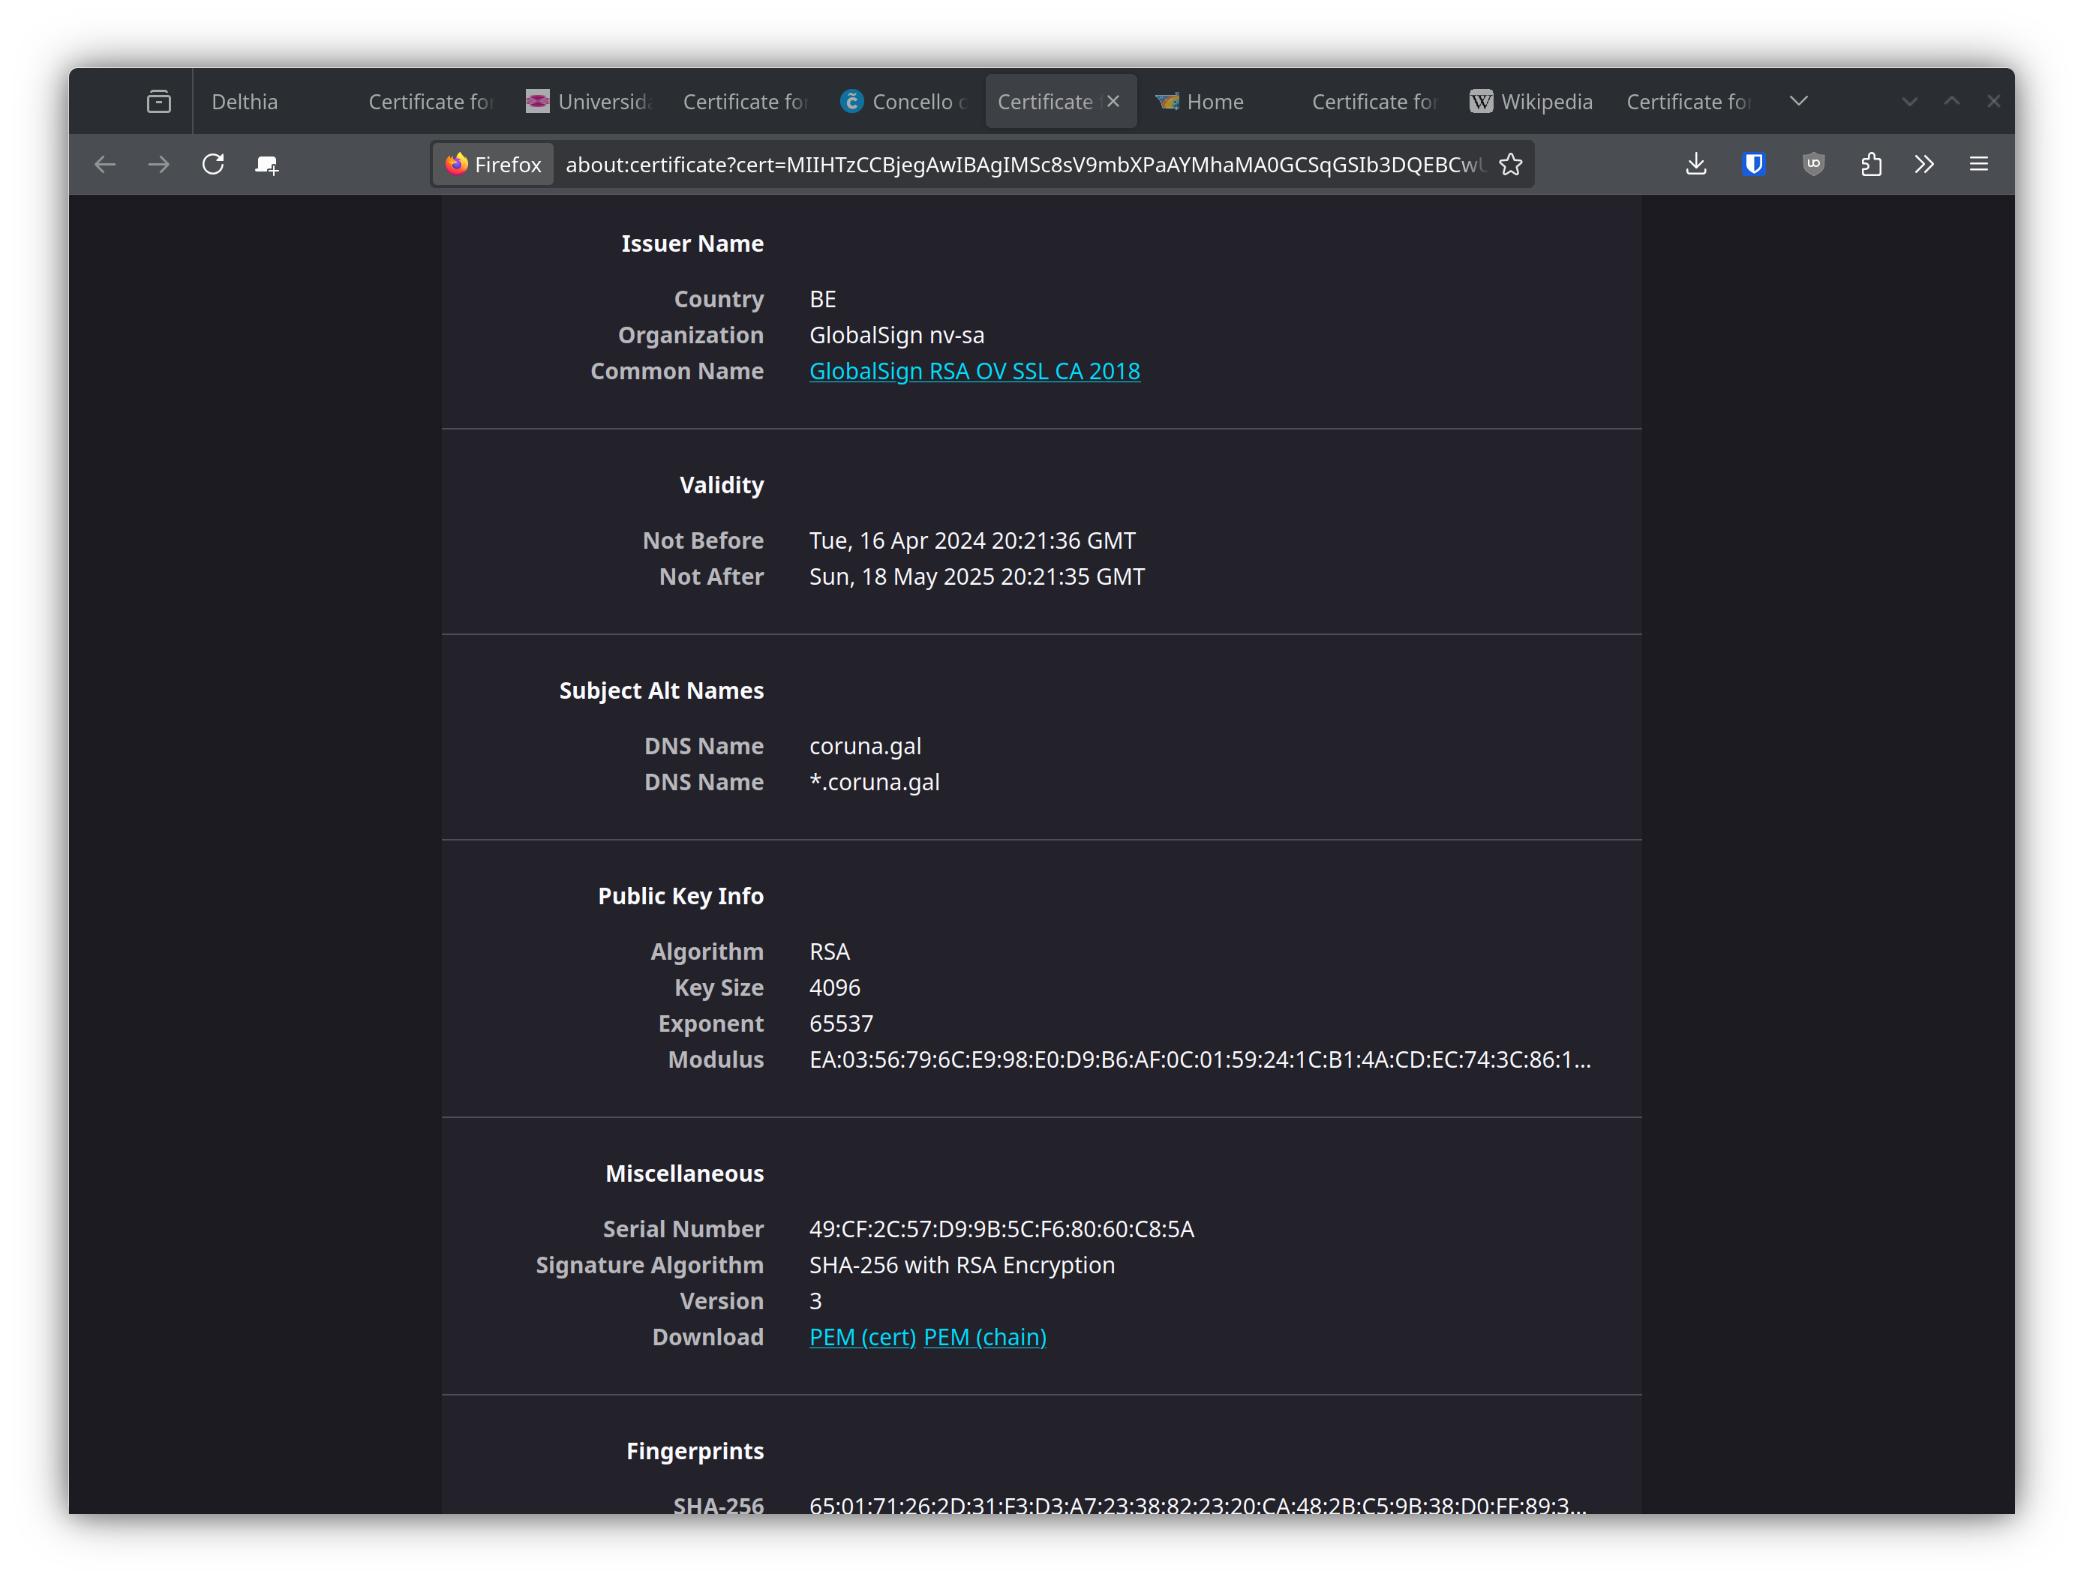
\includegraphics[width=0.8\textwidth]{cert-coruna.png}
    \caption{Certificado de \url{coruna.gal}}
\end{figure}

\begin{figure}[H]
    \centering
    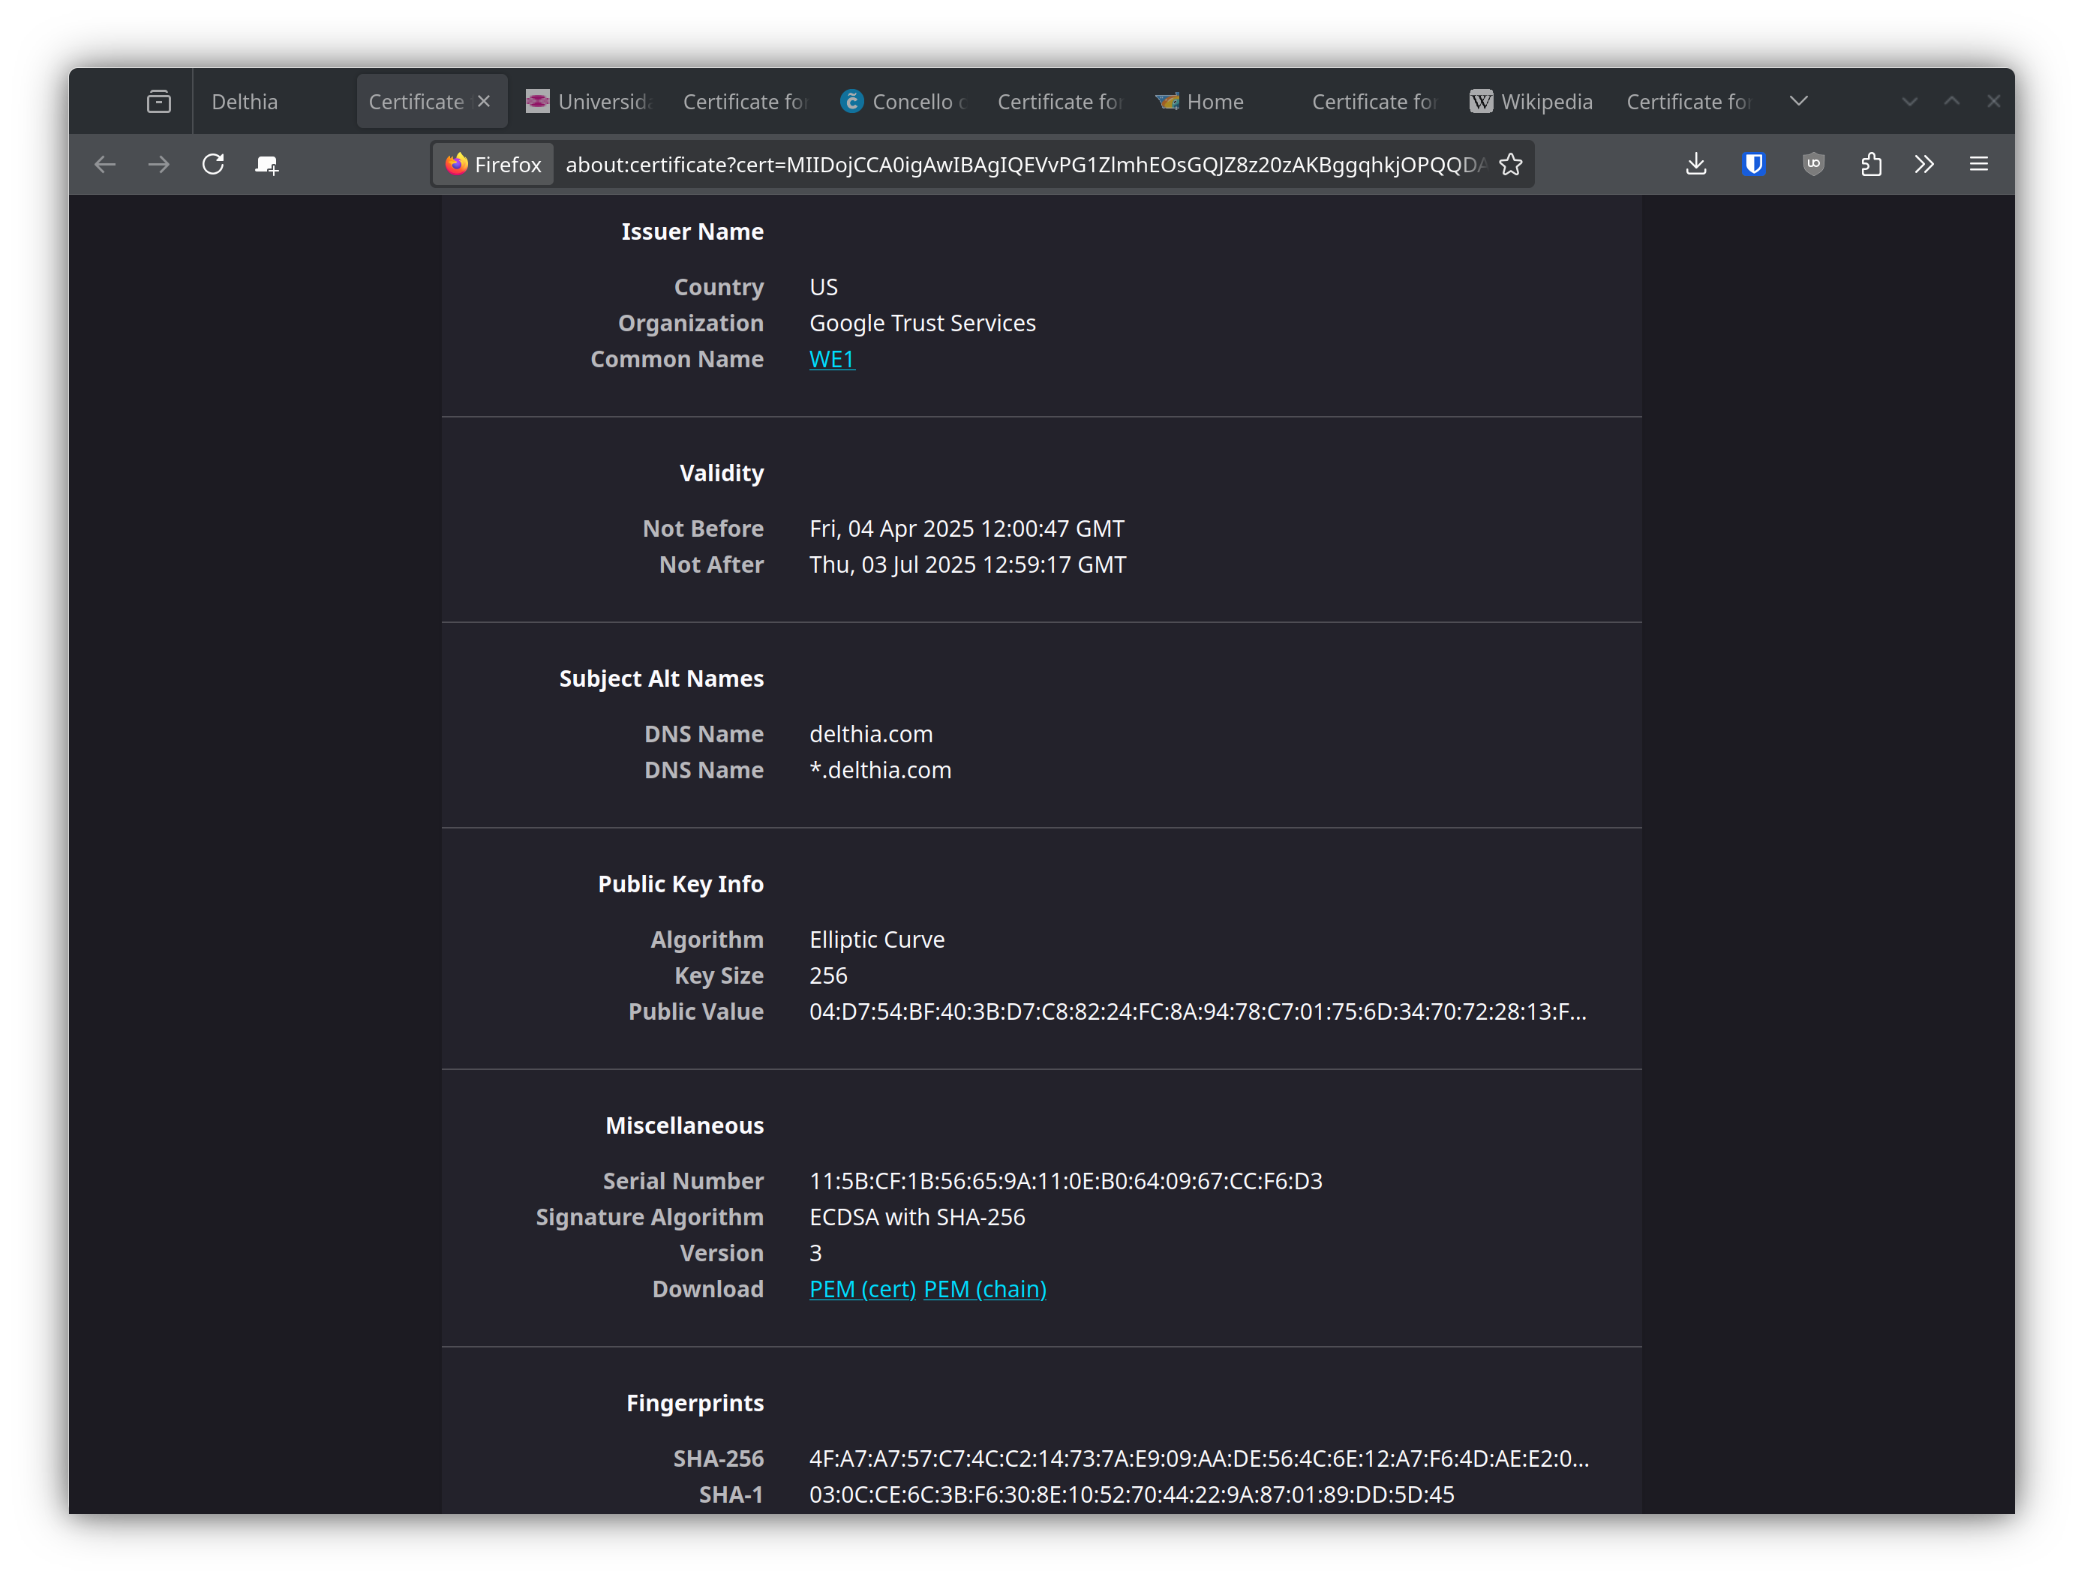
\includegraphics[width=0.8\textwidth]{cert-delthia.png}
    \caption{Certificado de \url{delthia.com}}
\end{figure}

\begin{figure}[H]
    \centering
    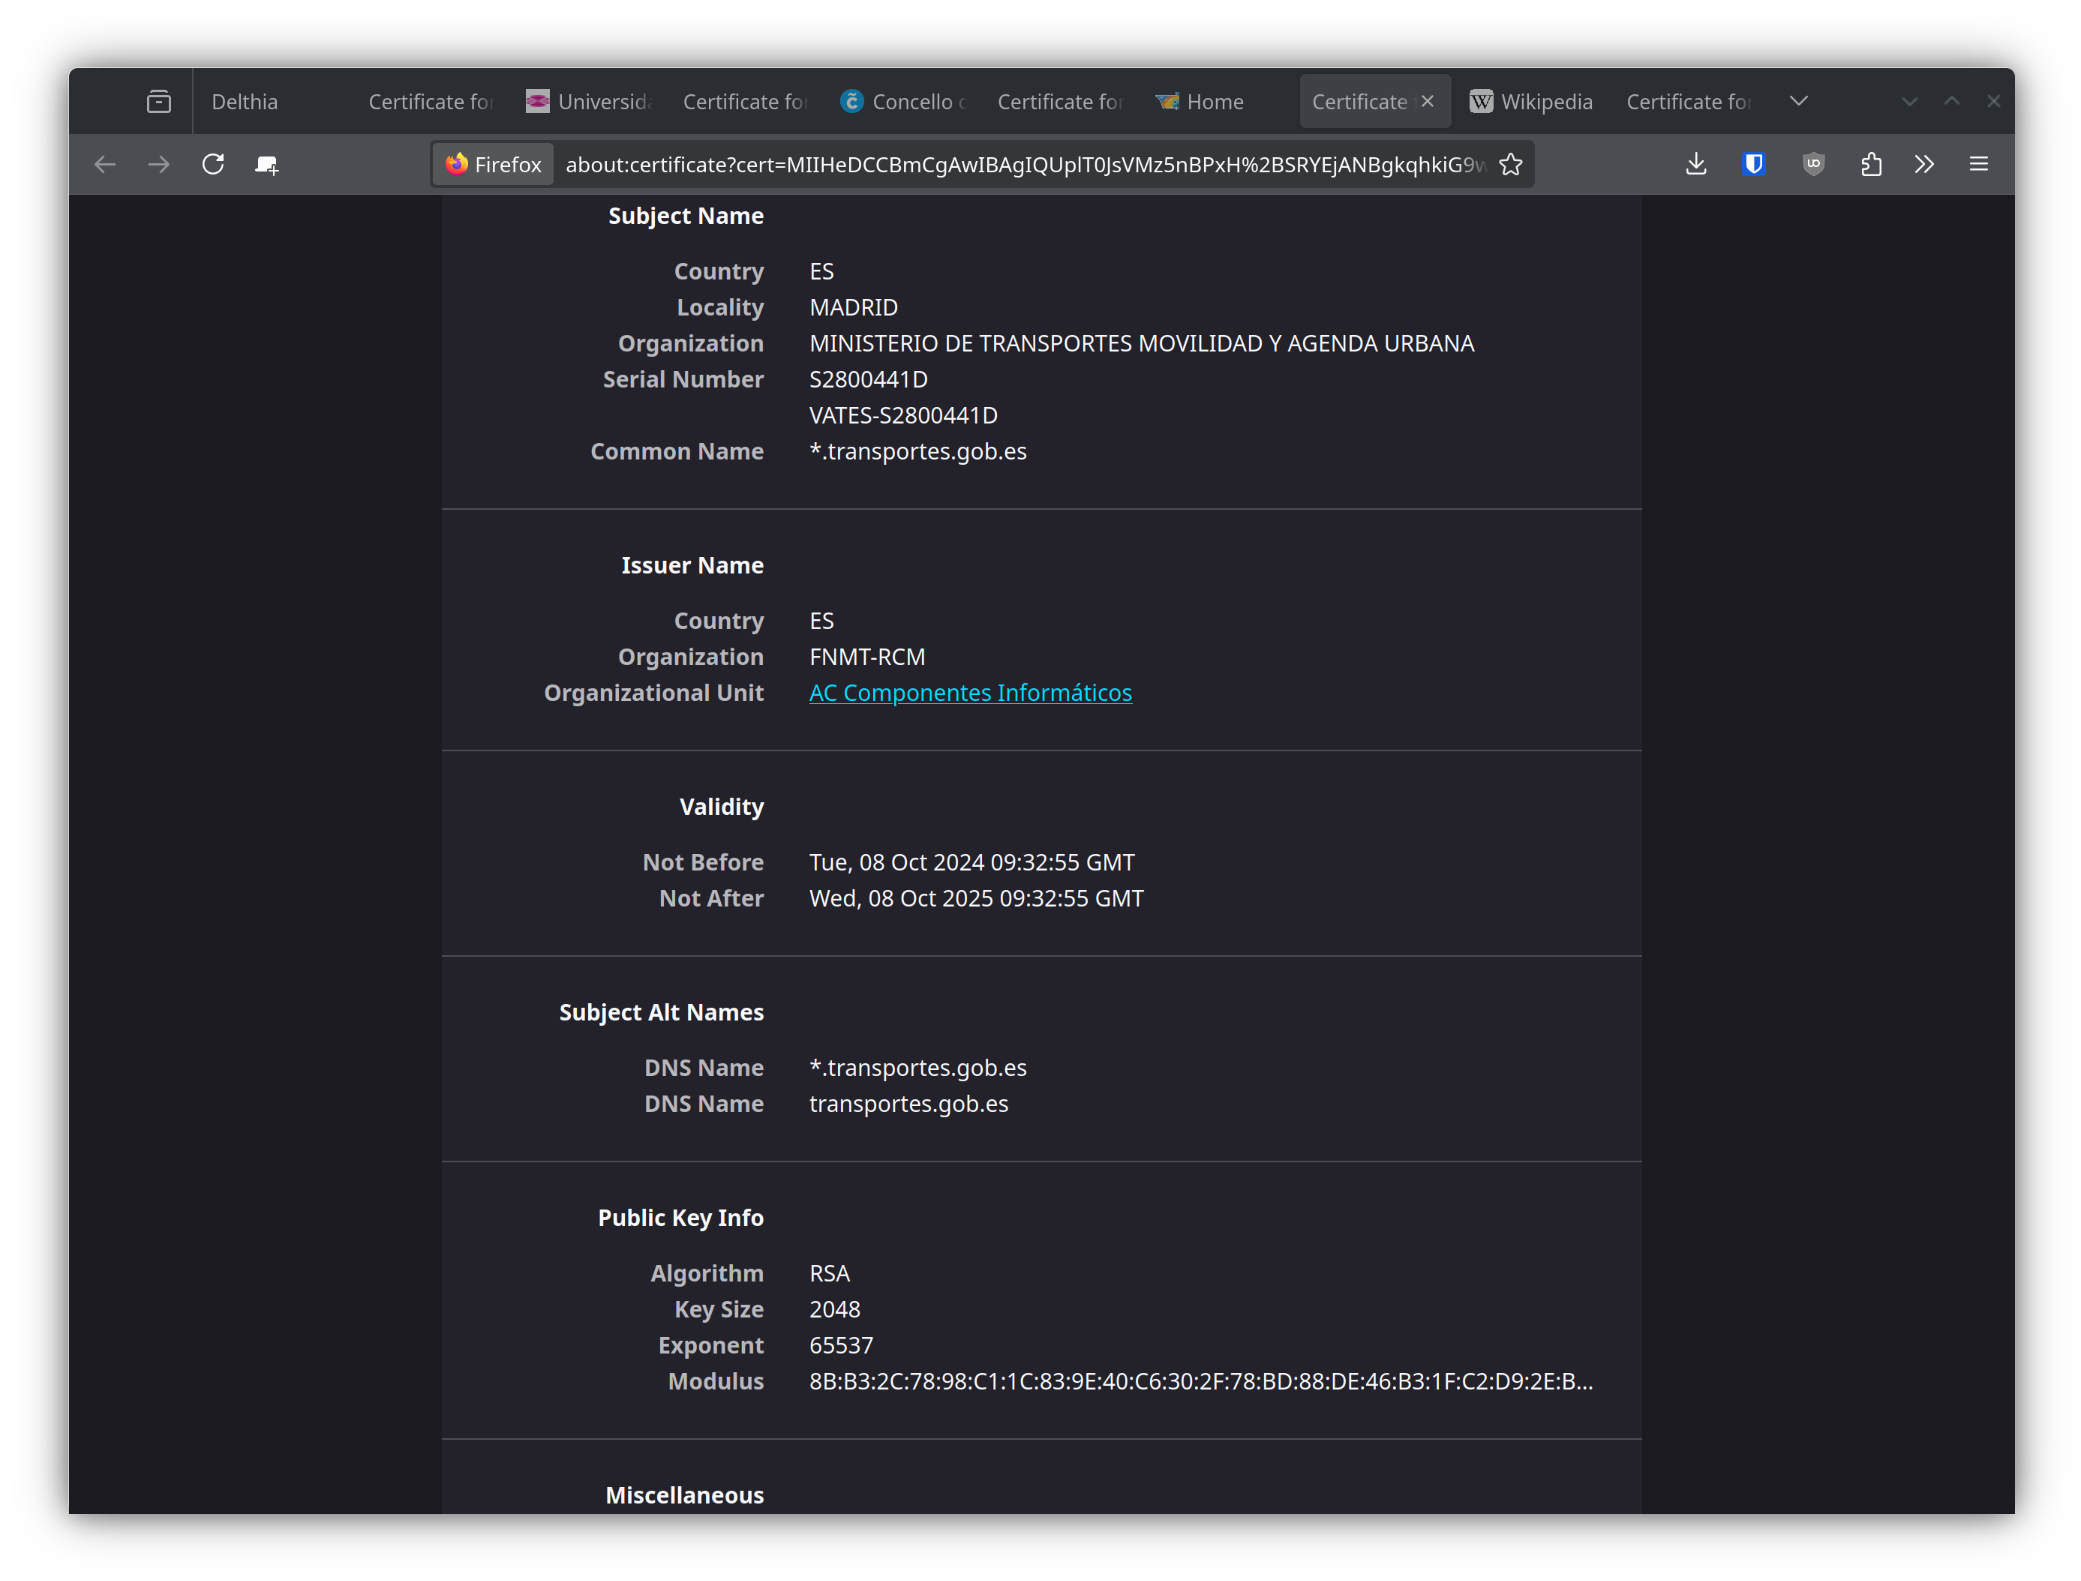
\includegraphics[width=0.8\textwidth]{cert-transportes.png}
    \caption{Certificado de \url{nap.transportes.gob.es}}
\end{figure}

\begin{figure}[H]
    \centering
    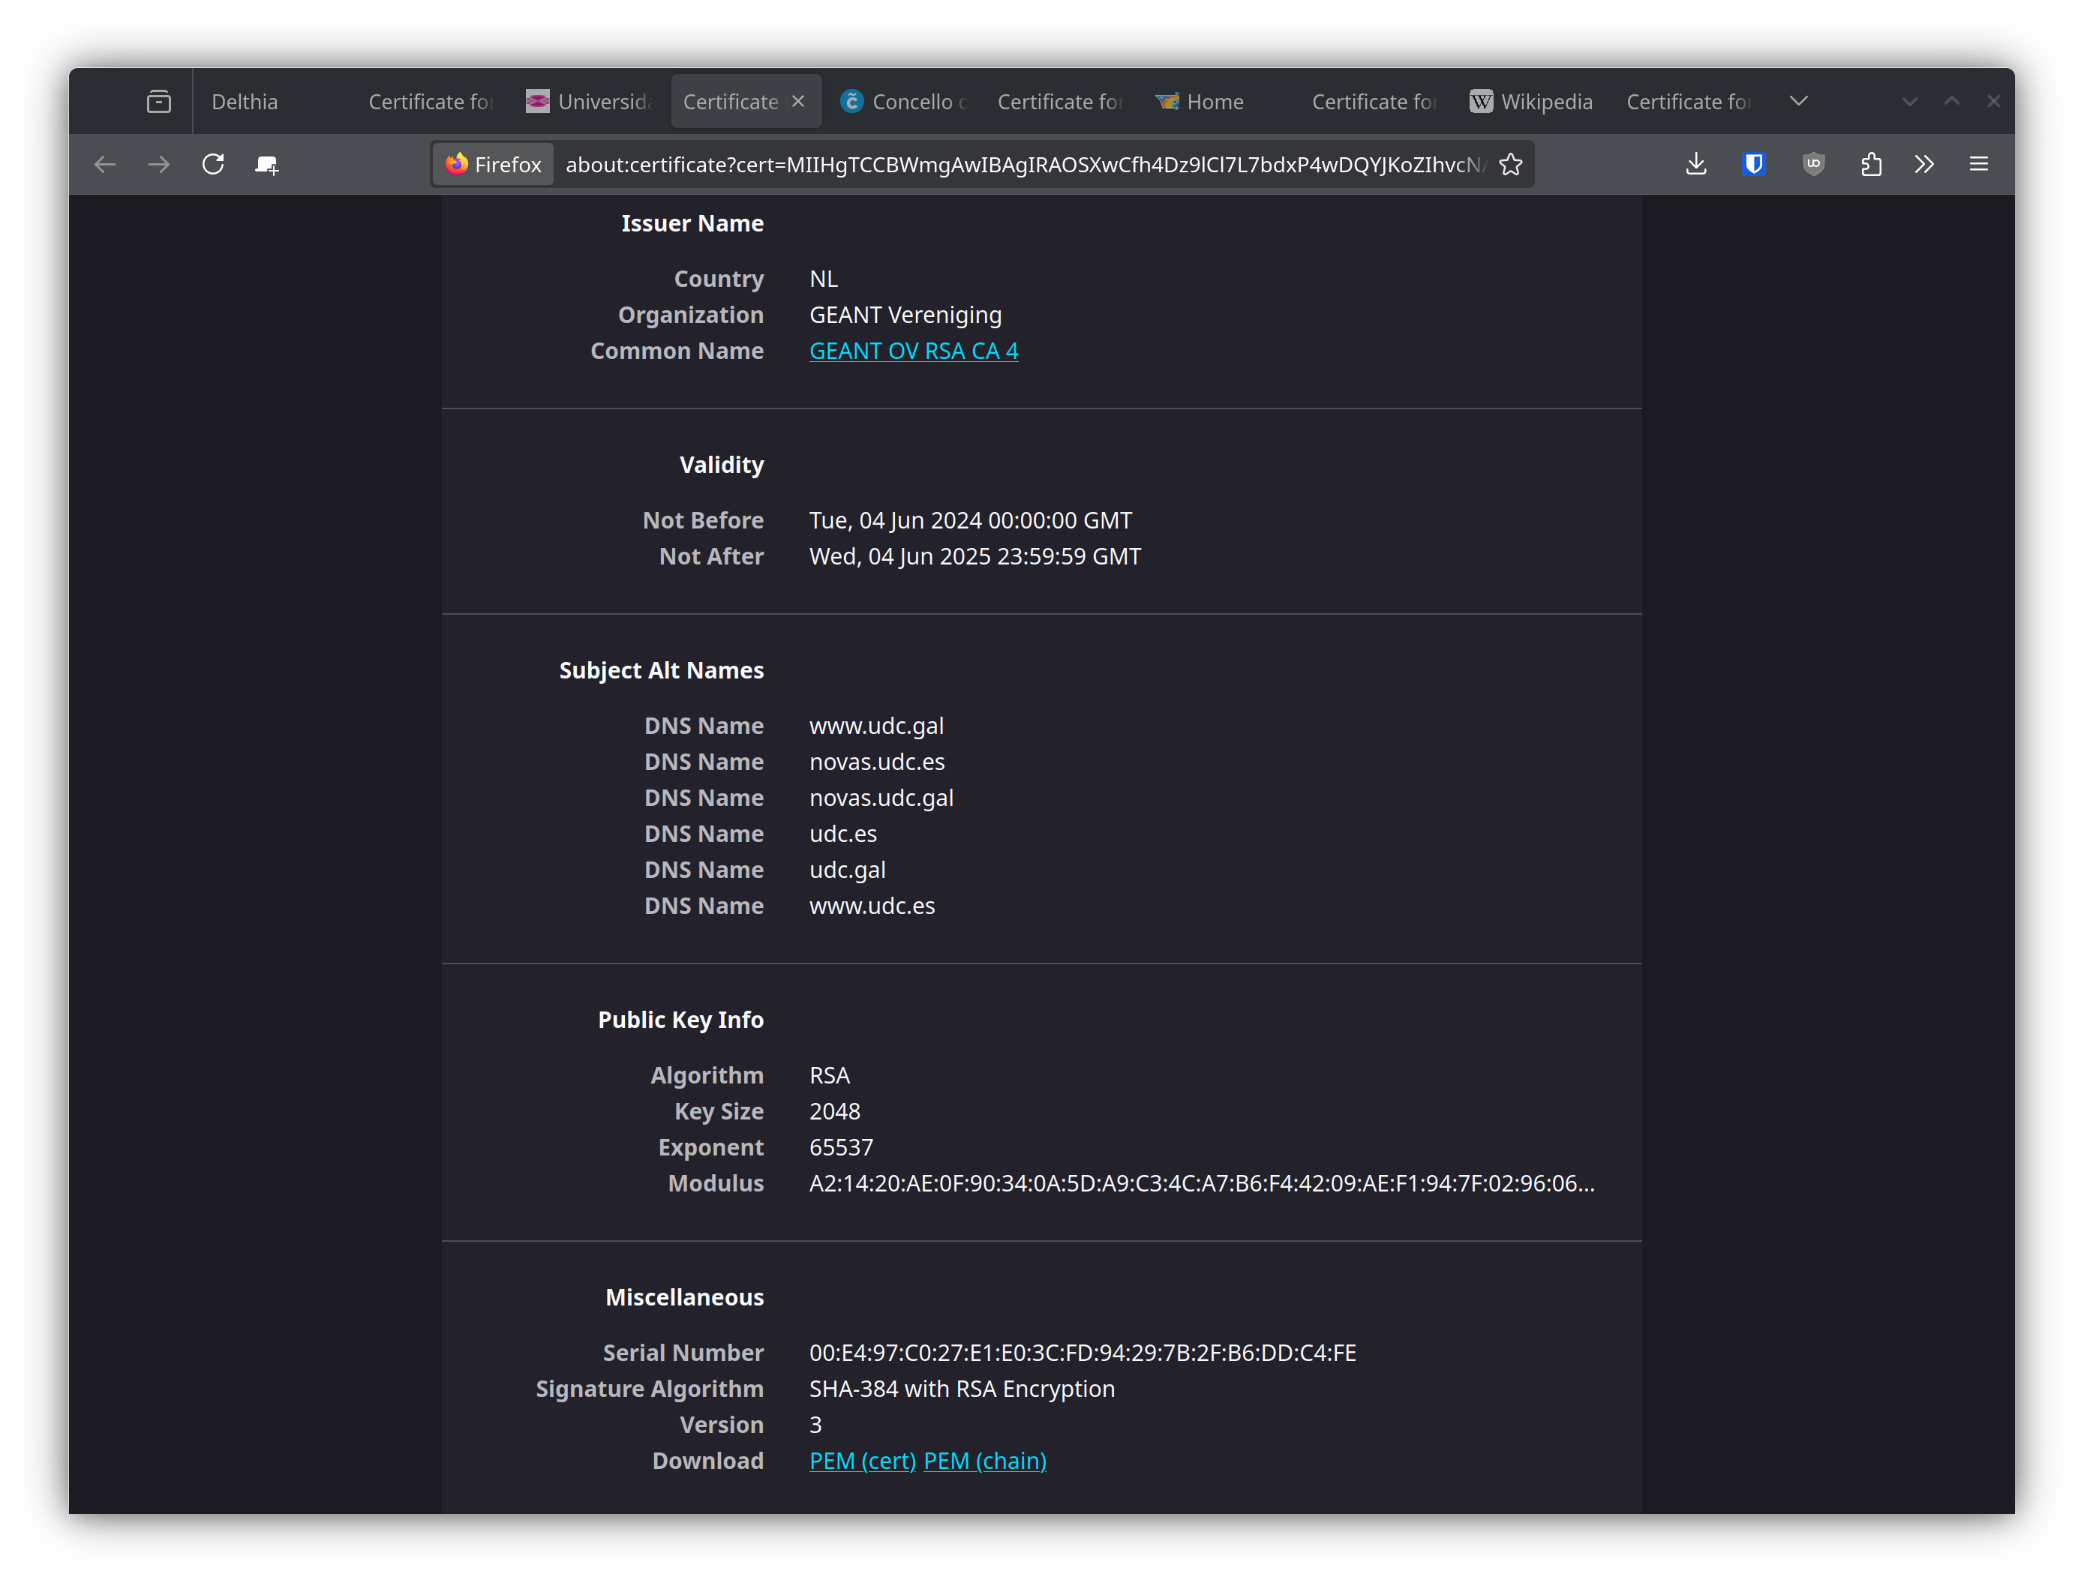
\includegraphics[width=0.8\textwidth]{cert-udc.png}
    \caption{Certificado de \url{udc.es}}
\end{figure}

\begin{figure}[H]
    \centering
    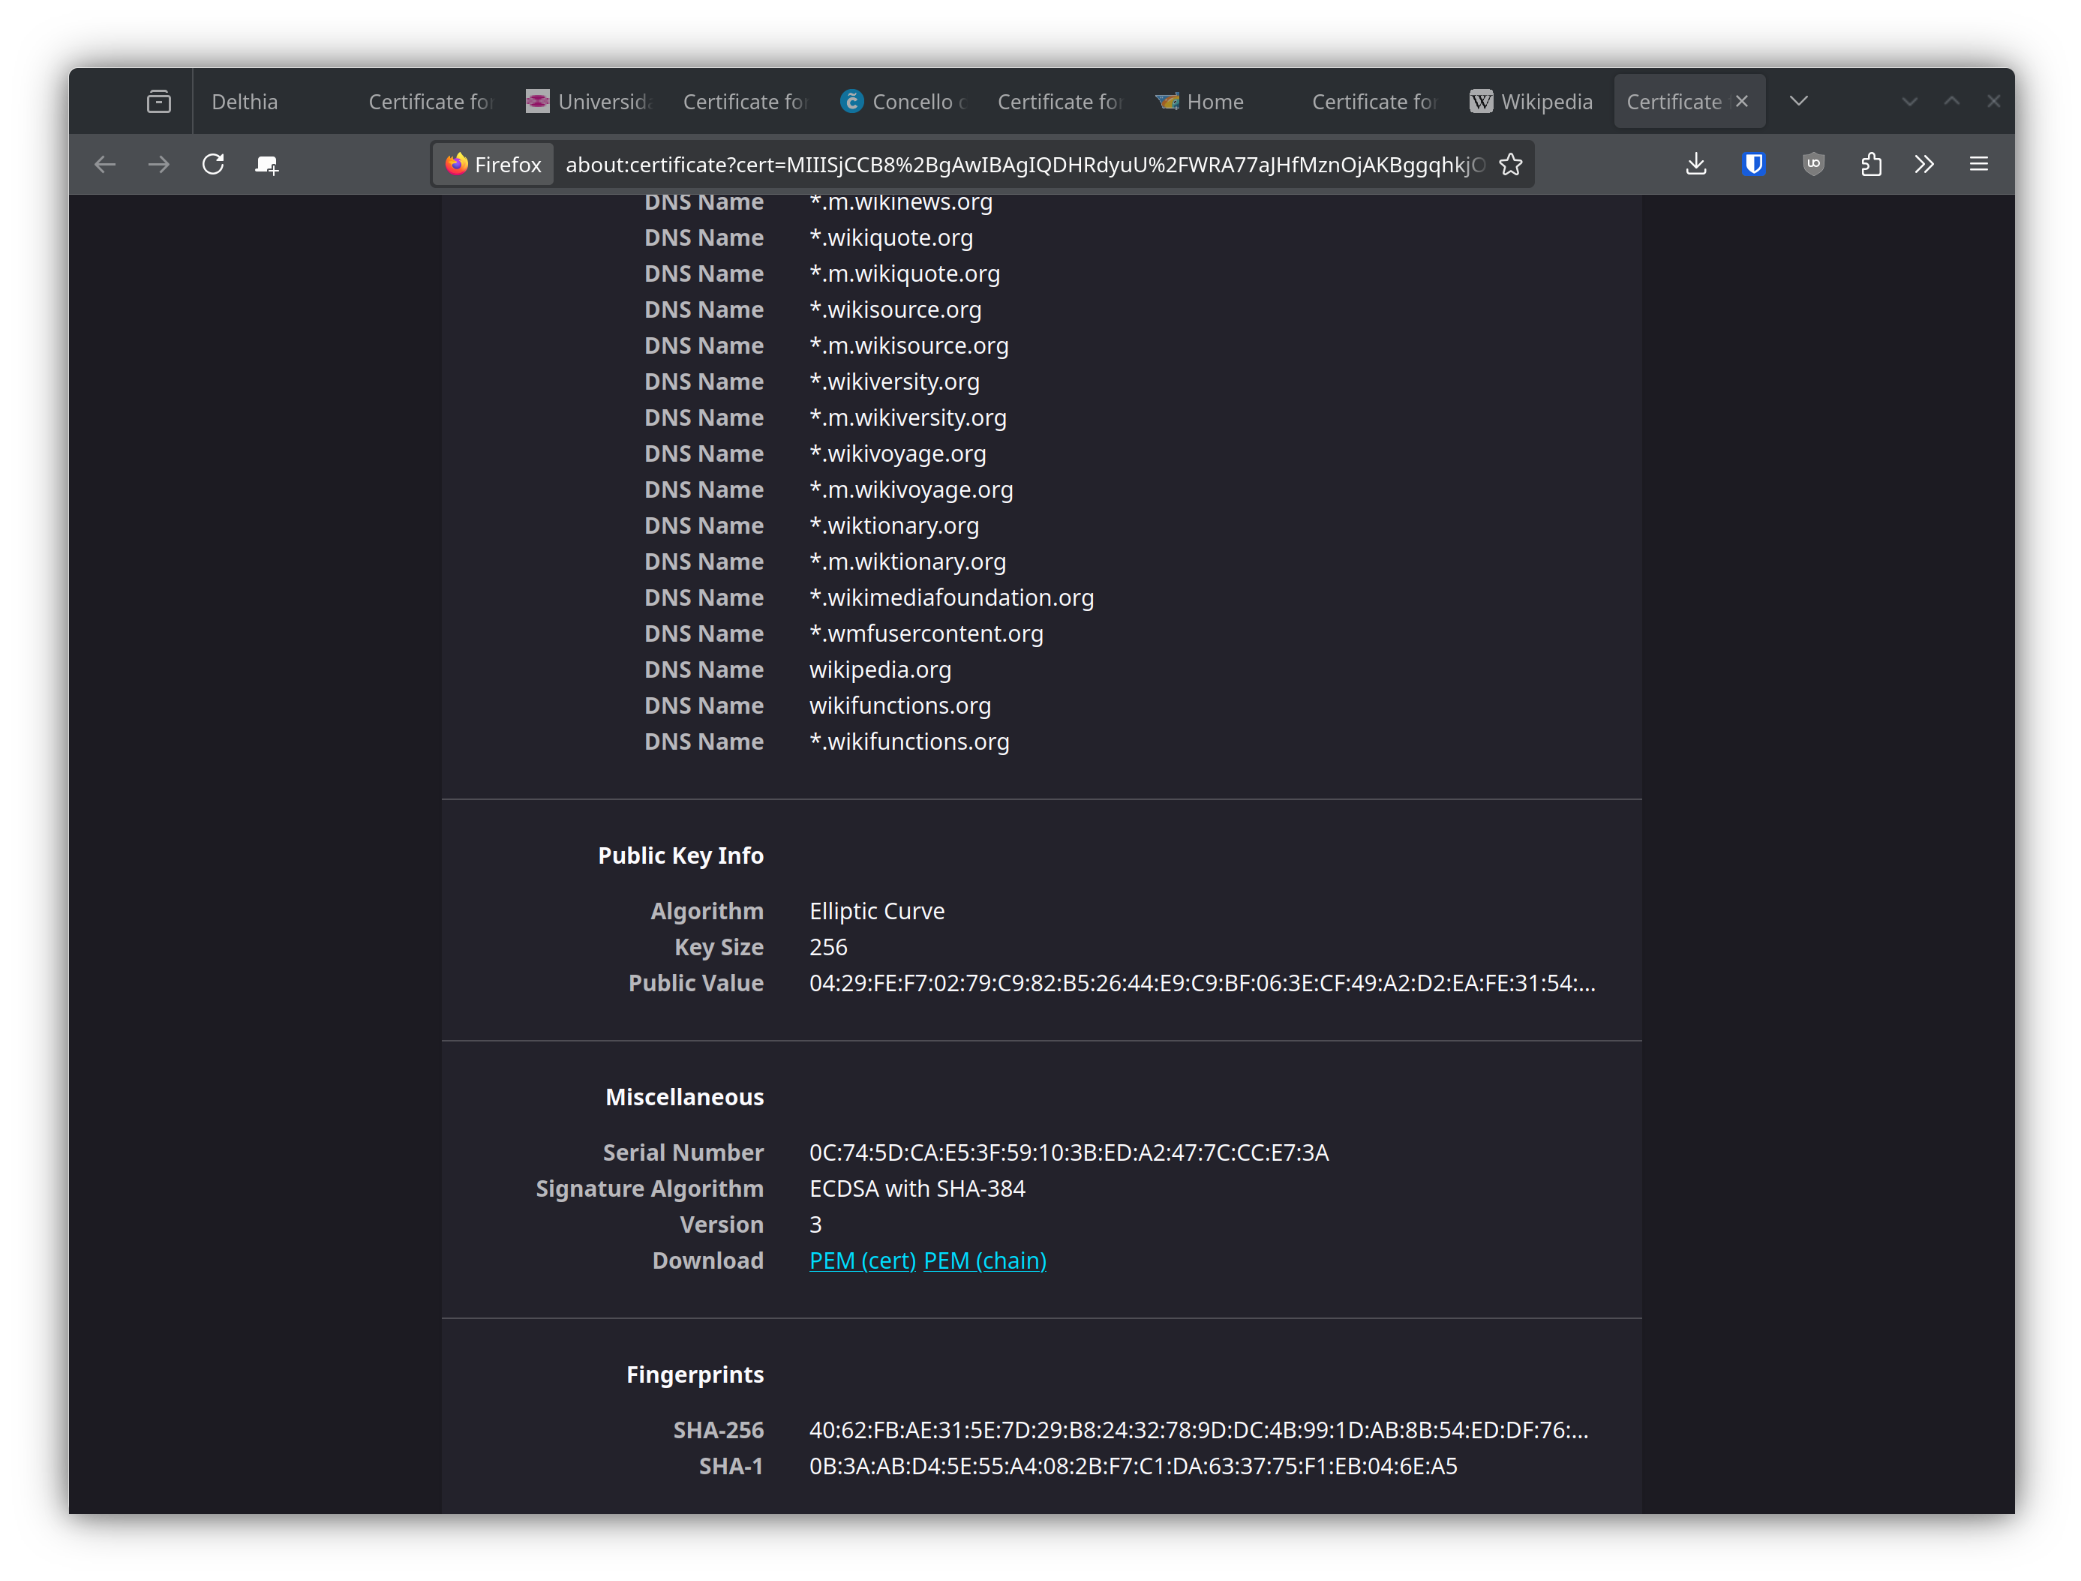
\includegraphics[width=0.8\textwidth]{cert-wikipedia.png}
    \caption{Certificado de \url{wikipedia.org}}
\end{figure}

\subsubsection{Análisis con openssl}

A continuación se analizan los certificados de \url{coruna.gal} y \url{udc.es}, para lo que utiliza \texttt{OpenSSL} ver los detalles del certificado descargado desde firefox.

\begin{minted}[
frame=single,
framesep=8pt,
breaklines,
bgcolor=bgGray,
]{bash}
    openssl x509 -in certificado.pem -text -noout
\end{minted}

\begin{figure}[H]
    \centering
    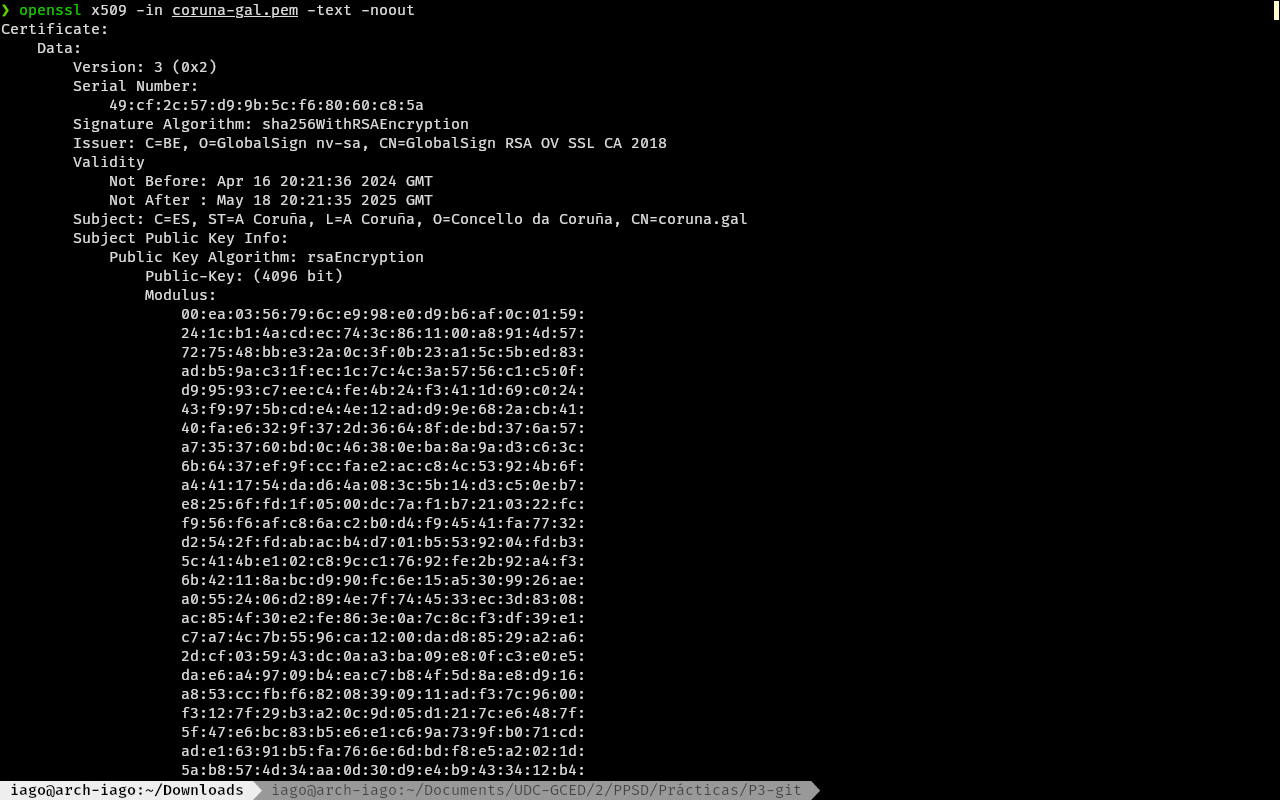
\includegraphics[width=0.8\textwidth]{openssl-coruna.png}
    \caption{Detalles del certificado de \url{coruna.gal}}
\end{figure}

En el caso de \url{coruna.gal} el certificado tiene como clave pública

\begin{minted}[
    frame=single,
    framesep=8pt,
    breaklines,
    bgcolor=bgGray
]{text}
00:ea:03:56:79:6c:e9:98:e0:d9:b6:af:0c:01:59:
24:1c:b1:4a:cd:ec:74:3c:86:11:00:a8:91:4d:57:
72:75:48:bb:e3:2a:0c:3f:0b:23:a1:5c:5b:ed:83:
ad:b5:9a:c3:1f:ec:1c:7c:4c:3a:57:56:c1:c5:0f:
d9:95:93:c7:ee:c4:fe:4b:24:f3:41:1d:69:c0:24:
43:f9:97:5b:cd:e4:4e:12:ad:d9:9e:68:2a:cb:41:
40:fa:e6:32:9f:37:2d:36:64:8f:de:bd:37:6a:57:
a7:35:37:60:bd:0c:46:38:0e:ba:8a:9a:d3:c6:3c:
6b:64:37:ef:9f:cc:fa:e2:ac:c8:4c:53:92:4b:6f:
a4:41:17:54:da:d6:4a:08:3c:5b:14:d3:c5:0e:b7:
e8:25:6f:fd:1f:05:00:dc:7a:f1:b7:21:03:22:fc:
f9:56:f6:af:c8:6a:c2:b0:d4:f9:45:41:fa:77:32:
d2:54:2f:fd:ab:ac:b4:d7:01:b5:53:92:04:fd:b3:
5c:41:4b:e1:02:c8:9c:c1:76:92:fe:2b:92:a4:f3:
6b:42:11:8a:bc:d9:90:fc:6e:15:a5:30:99:26:ae:
a0:55:24:06:d2:89:4e:7f:74:45:33:ec:3d:83:08:
ac:85:4f:30:e2:fe:86:3e:0a:7c:8c:f3:df:39:e1:
c7:a7:4c:7b:55:96:ca:12:00:da:d8:85:29:a2:a6:
2d:cf:03:59:43:dc:0a:a3:ba:09:e8:0f:c3:e0:e5:
da:e6:a4:97:09:b4:ea:c7:b8:4f:5d:8a:e8:d9:16:
a8:53:cc:fb:f6:82:08:39:09:11:ad:f3:7c:96:00:
f3:12:7f:29:b3:a2:0c:9d:05:d1:21:7c:e6:48:7f:
5f:47:e6:bc:83:b5:e6:e1:c6:9a:73:9f:b0:71:cd:
ad:e1:63:91:b5:fa:76:6e:6d:bd:f8:e5:a2:02:1d:
5a:b8:57:4d:34:aa:0d:30:d9:e4:b9:43:34:12:b4:
ec:01:72:bc:6f:9c:93:f6:35:d0:12:3b:66:b6:5e:
d5:a5:c2:e2:c7:ec:4f:ec:5e:c5:d4:4d:ec:e0:23:
f3:70:79:a6:af:5f:d7:cc:16:b8:48:f7:2d:90:93:
37:97:99:17:4e:47:54:5a:af:ce:7f:2e:2a:22:4d:
f7:a1:c1:94:48:75:b6:23:04:da:32:3b:13:5c:c3:
44:9d:8a:80:d8:0a:0b:c6:51:c9:35:93:42:d4:44:
ba:75:95:38:16:36:13:46:25:2c:36:fc:02:fd:af:
87:bd:26:29:a1:97:dd:e9:e8:cc:dd:74:98:38:4b:
5d:fb:52:3c:46:52:04:01:72:81:c5:78:e8:0c:ee:
3a:1a:85
\end{minted}

cuya representación en decimal es:

\begin{minted}[
    frame=single,
    framesep=8pt,
    breaklines,
    bgcolor=bgGray
]{text}
954689903308970528555674972115139987855010150
900611376489209355409562145324116437915059655
899610442406373930674332180554390635358347993
391847689718920650807233623377503920363718955
675671725539504773298126523495908191801703959
831780960130049520620198901661036653851941666
949840543611794979186288997467344743507524701
229284045793976527052528003774365802970981367
696103998511136745763933537083048735501325575
046495265040858009999219024046651055374139391
643133586764444519875748198451241089493320137
744371821910482740616757707579843269732768550
692644940331906094503515716630550662511876576
965457277175613712180378774472024422861557006
811462686700601076333907540724996766442827933
177601342052045294288075615158618920387837314
955504508632543337764765943506762895356189387
814457471653592362617546188827583373506698569
572625888645440322333187143971013979030956193
279002248929904934870939128713065790306154332
938853267833200816077256552087297530032584388
149938235291809430599150895081926322635223983
737369849126339195981853565008656264635851206
576536463141179887852282135526981442570082334
062902425388641223857215021804461105519741322
487508485027503896101433947218272729710914025
976741214206227600671140625962511938686664541
809749638417881733
\end{minted}

Además, el valor del Common Name es \texttt{coruna.gal} y lo emitió GlobalSign: \texttt{Issuer: C=BE, O=GlobalSign nv-sa, CN=GlobalSign RSA OV SSL CA 2018}.

\begin{figure}[H]
    \centering
    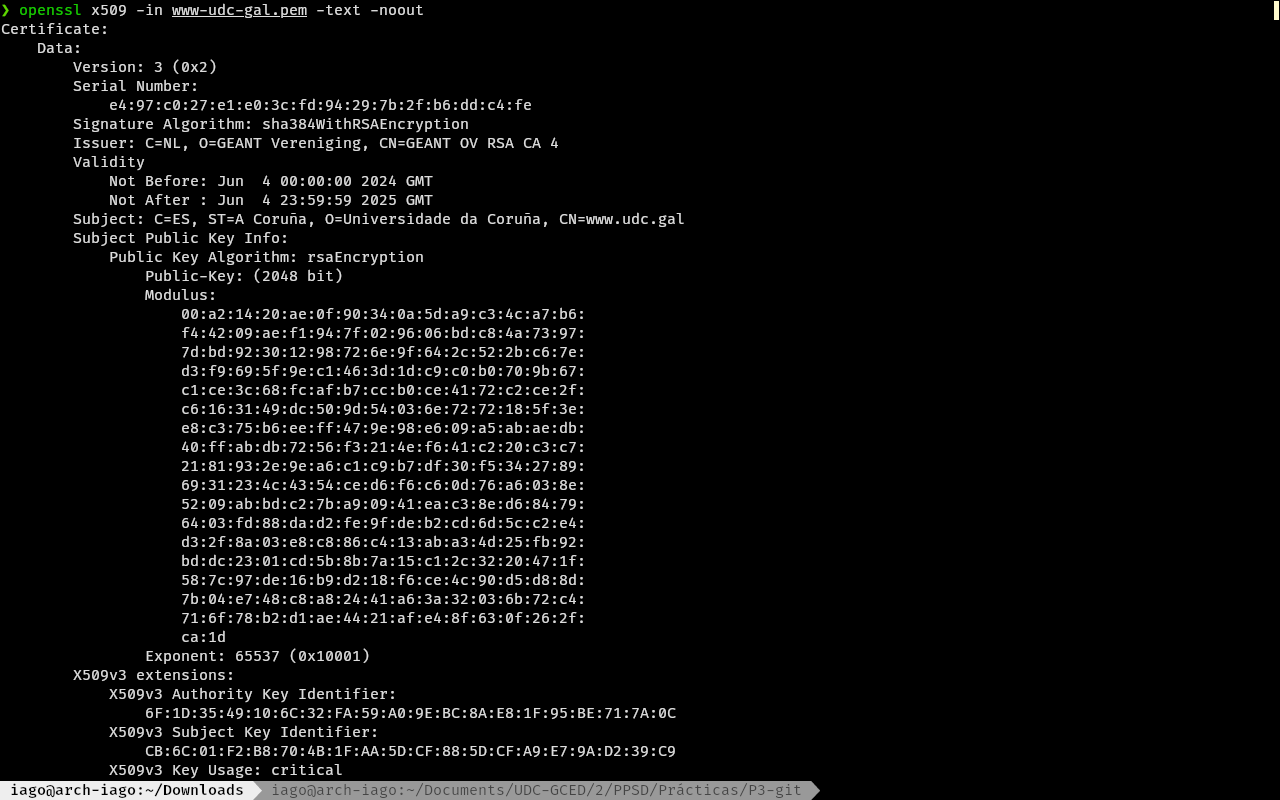
\includegraphics[width=0.8\textwidth]{openssl-udc.png}
    \caption{Detalles del certificado de \url{www.udc.es}}
\end{figure}

En el caso de \url{udc.gal} el certificado tiene como clave pública

\begin{minted}[
    frame=single,
    framesep=8pt,
    breaklines,
    bgcolor=bgGray
]{text}
00:a2:14:20:ae:0f:90:34:0a:5d:a9:c3:4c:a7:b6:
f4:42:09:ae:f1:94:7f:02:96:06:bd:c8:4a:73:97:
7d:bd:92:30:12:98:72:6e:9f:64:2c:52:2b:c6:7e:
d3:f9:69:5f:9e:c1:46:3d:1d:c9:c0:b0:70:9b:67:
c1:ce:3c:68:fc:af:b7:cc:b0:ce:41:72:c2:ce:2f:
c6:16:31:49:dc:50:9d:54:03:6e:72:72:18:5f:3e:
e8:c3:75:b6:ee:ff:47:9e:98:e6:09:a5:ab:ae:db:
40:ff:ab:db:72:56:f3:21:4e:f6:41:c2:20:c3:c7:
21:81:93:2e:9e:a6:c1:c9:b7:df:30:f5:34:27:89:
69:31:23:4c:43:54:ce:d6:f6:c6:0d:76:a6:03:8e:
52:09:ab:bd:c2:7b:a9:09:41:ea:c3:8e:d6:84:79:
64:03:fd:88:da:d2:fe:9f:de:b2:cd:6d:5c:c2:e4:
d3:2f:8a:03:e8:c8:86:c4:13:ab:a3:4d:25:fb:92:
bd:dc:23:01:cd:5b:8b:7a:15:c1:2c:32:20:47:1f:
58:7c:97:de:16:b9:d2:18:f6:ce:4c:90:d5:d8:8d:
7b:04:e7:48:c8:a8:24:41:a6:3a:32:03:6b:72:c4:
71:6f:78:b2:d1:ae:44:21:af:e4:8f:63:0f:26:2f:
ca:1d
\end{minted}

cuya representación en decimal es:

\begin{minted}[
    frame=single,
    framesep=8pt,
    breaklines,
    bgcolor=bgGray
]{text}
204605307215754979258097502582964693603000409
126578374083369809657669638883649487005490957
272184329823665985208197591736691516362494915
843448924180180245184795770879876282610161126
366046675881799907238489522997638750937333091
438644139765326173630674432956998856134857109
550036461707384379691772677552427943001221107
365795171149741997673537438148871340536956612
564726058816573266996948186798429478922472547
202925244696383650575097034085490026365004601
929629217976773800487595249957362910022580003
356153311949020181342484727491249102712835428
006028240438832185860024359730206746365092441
47296969328241437258920563296797
\end{minted}

Además, el valor del Common Name es \texttt{www.udc.gal} y lo emitió GEANT: \texttt{Issuer: C=NL, O=GEANT Vereniging, CN=GEANT OV RSA CA 4}.

\subsubsection{Importancia Common Name}

El Common Name es el campo que indica el nombre de dominio para el que es válido el certificado. Representa un nombre general del servidor, generalmente el subdominio de menor nivel para el que es válido, ya que en el certificado se pueden indicar más subdominios (o incluso dominios) para los que es válido en el campo de nombres alternativos.
